\subsection{Product Perspective}
\subsubsection{Scenarios}
\begin{enumerate}
    \item \textbf{Educator creates a battle for a tournament} \\
    The educator who wants to create a battle in a tournament for which he is the creator, or for which he has the permission to create battles.
    The creation of a battle consists of in:
    \begin{itemize}
        \item Set the deadline for registration of teams
        \item Set the deadline for the submission of solutions
        \item Set the minimum and maximum number of students per team
        \item Upload the code kata to the CKB platform
    \end{itemize}
    Once the battle is created, the students registered at that tournament are notified by CKB about the upcoming battle. The CKB platform will also create a new repository on Github for the battle, and will invite the students to fork it.
    \item \textbf{Student invite other students to join the team} \\
    Roberto is a student who wants to participate in a battle. He has already registered in the tournament in which the battle has been created, and he has been notified about the upcoming battle. He wants to invite other students to join his team for the battle. He can do this by sending an invitation to the other students, who will receive a notification about the invitation. The other students can accept or decline the invitation. If they accept, they will be added to the team and they will be able to compete as a team in a battle.
    Even if the students invited have accepted the invitation the partecipation to the battle is not guaranteed since the educator could have set a maximum number of students per team.
    \item \textbf{Student push the solution of the battle to the forked repository} \\
    The team A have been working on the solution for the battle for a while and it seems to be passing all the tests provided in the code kata. Since the time being is before the submission deadline the team push the solution to the forked repository. This will trigger the CKB platform to evaluate the solution and update the score of the team in the battle. In the case that the submission date is after the submission deadline the push will not trigger another evaluation of the solution by the CKB platform.
    \item \textbf{Educator manually updates the score of a team} \\
    Giacomo is an educator who has created a battle for a tournament in which he has been invited by another collegue. Once the submission deadline is expired he wants to manually assess the score of a team to cover all the aspects that the CKB platform cannot evaluate. To do this he access through the CKB platform the battle page and he can see the list of teams that have submitted a solution. He can then manually update the score of a team by clicking on the `Update score' button. This will open a form where he can modify the current score of the team previously evaluated by the platform. Once he is satisfied with the score he can click on the `Save' button to save the new score for the team. The new score will be visible to the team and to the other students subscribed to the tournament.
    \item \textbf{CKB notifies students about the result of the tournament} \\
    When an Educator closes a tournament, the CKB platform will notify all the students subscribed to the tournament about the result of the tournament. The notification will contain the list of the teams that have participated in the tournament and their final score.

\end{enumerate}
\subsubsection{Domain class Diagram}
\begin{figure}[H]
    \centering
    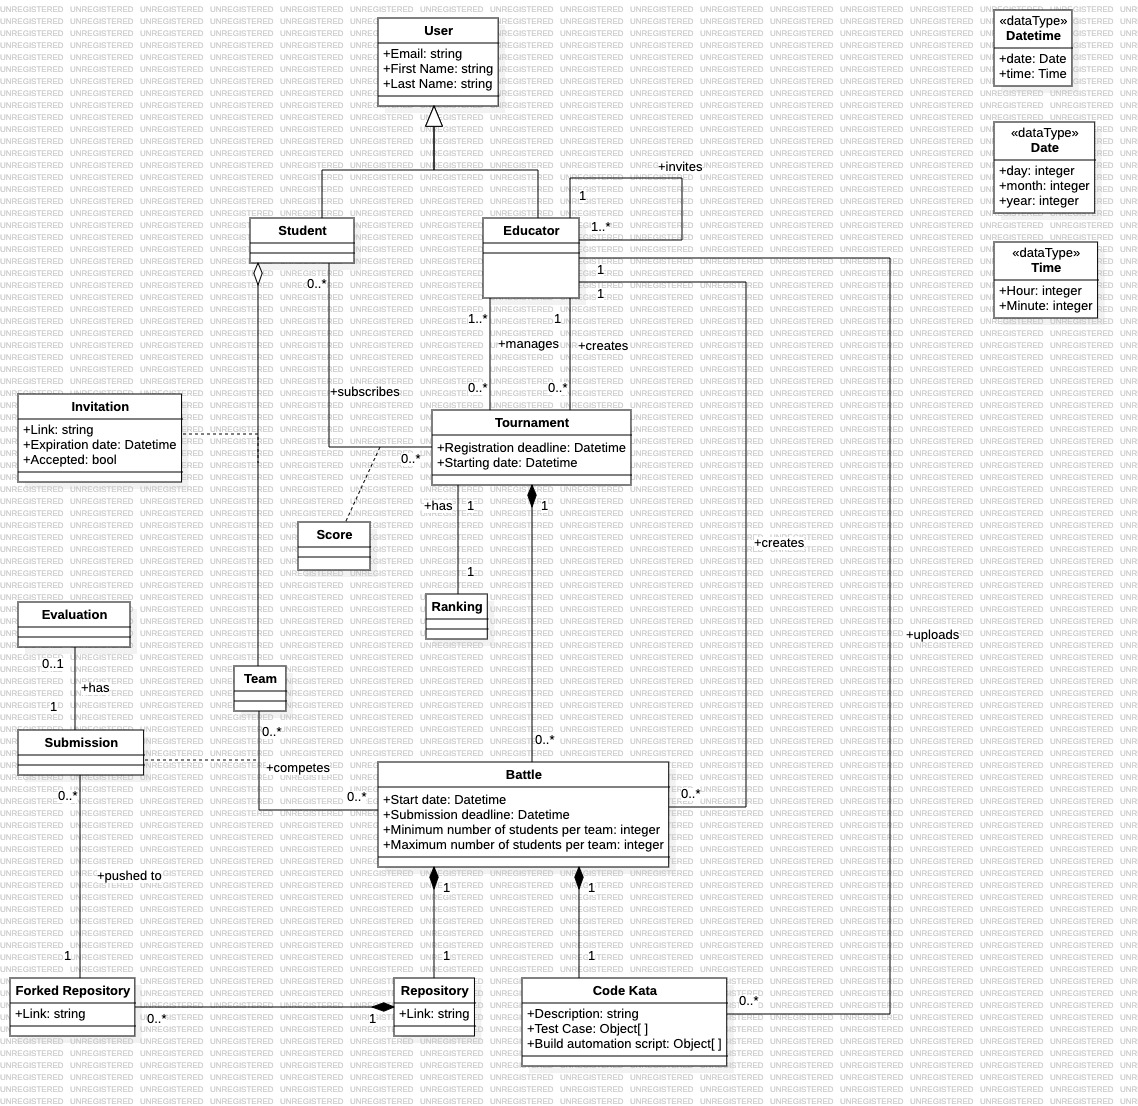
\includegraphics[width=1\textwidth]{Diagrams/DomainClassDiagram.jpg}
    \caption{Domain class diagram}
    \label{fig:domain_class_diagram}
\end{figure}